\chapter{BDD partie 1}
\section{Introduction}
\subsection{BDD et SGBD}
Une \textit{base de données} (BDD) est un ensemble structuré de données ainsi que des relations logiques sur ces données.\\

Le \textit{système de gestion de bases de données} (SGBD) peut être vu comme le logiciel qui gère :
\begin{itemize}
    \item	la structuration des données ;
    \item	le stockage des données ;
    \item 	la maintenance des données ;
    \item 	la sécurité des données ;
    \item 	les accès aux données (lecture et/ou écriture) en temps réel par de multiples intervenants.
\end{itemize}


\subsection{Un peu d'histoire}
La majorité de ce que nous allons voir repose sur les travaux d'Edgar F. Codd, c'est lui qui a inventé le modèle relationnel en 1970 alors qu'il travaillait comme informaticien chez IBM.
\begin{center}
    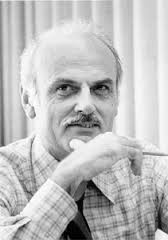
\includegraphics[width=3cm]{img/codd}
\end{center}


\subsection{Phases de conception d'une BDD}
C'est une tâche essentielle pour assurer le bon fonctionnement des applications qui vont l'utiliser.
\begin{itemize}
    \item	\textit{niveau conceptuel} : on représente la BDD à l'aide de schémas indépendamment de toute considération informatique ;
    \item	\textit{niveau logique} on adapte le schéma en tables à deux dimensions ;
    \item	\textit{niveau physique} on implémente les tables sur un SGBD.
\end{itemize}

\section{Niveau conceptuel : modèle entités-associations}
\subsection{Entités}
On commence par déterminer les types des entités qui interviennent:
\begin{itemize}
    \item	une \textit{entité} est un objet unique avec un nombre fini d'attributs ;
    \item	un (ou plusieurs) attribut(s) permet(tent) d'identifier de manière unique l'entité : on parle d'\textit{identifian}t(s) ou de clé.
\end{itemize}
\begin{center}
    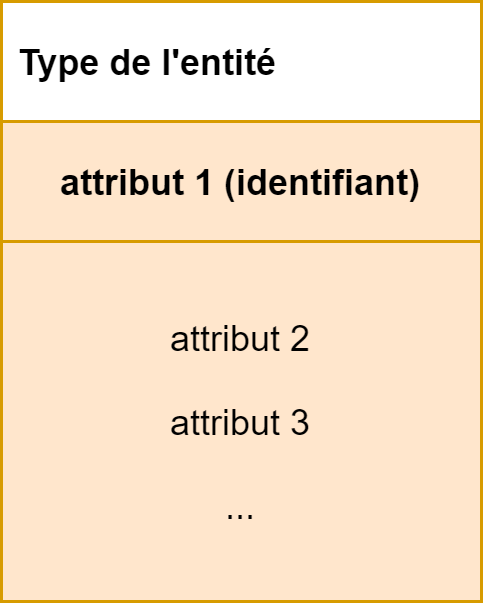
\includegraphics[width=3cm]{img/entité}
\end{center}

\begin{exemple}[ : entité-type Auteur]
    \begin{center}
        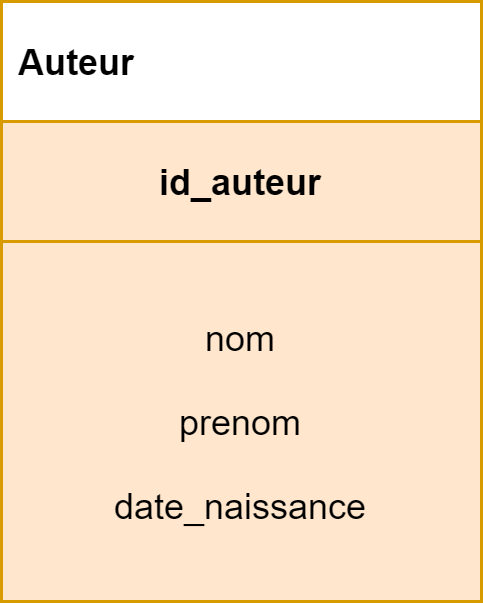
\includegraphics[width=3cm]{img/auteur}
    \end{center}
\end{exemple}
\subsection{Occurrences}

Une entité-type a en général plusieurs occurrences, appelées entités.\\

\begin{center}
    \tabstyle[UGLiBlue]
    \begin{tabular}{cccc}
        \hline
        
        \ccell{id\_auteur } & \ccell{nom} & \ccell{prenom} & \ccell{date\_naissance} \\\hline
        00000001            & Dupond      & Marie          & 23/08/1982              \\
        12345678            & Martin      & Luce           & 13/05/1963              \\
        98765432            & Leblanc     & Jean           & 18/11/1974              \\
        \hline
    \end{tabular}
\end{center}
\begin{remarque}
    Par souci de simplicité, on parlera d'entité à la fois pour désigner l'entité-type et chacune de ses occurrences.
\end{remarque}

\subsection{Entité Pays}
Voici une autre entité entrant en jeu dans la BDD :
\begin{center}
    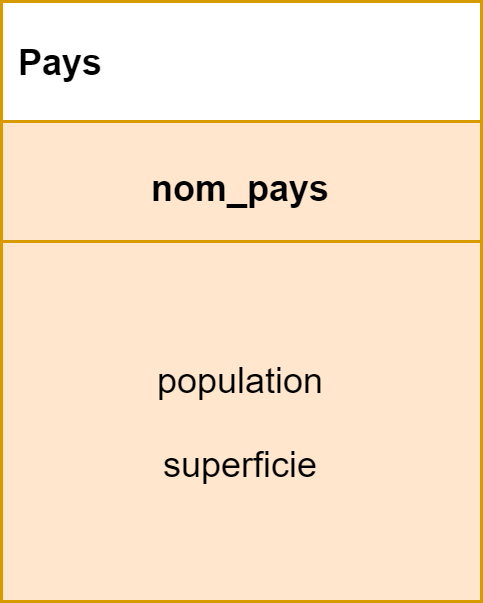
\includegraphics[width=3cm]{img/pays}
\end{center}


\subsection{Associations}
Elles définissent des \textit{liens sémantiques} (des liens de sens)	 que les simples entités ne suffisent pas à définir.\\

Une association comporte :
\begin{itemize}
    \item	un nom;
    \item 	un lien entre 2 relations ;
    \item	deux cardinalités qui sont représentées sur les extrémités du lien ;
    \item 	parfois elle peut comporter un ou des attributs.
\end{itemize}

\begin{exemple}[]
    \begin{center}
        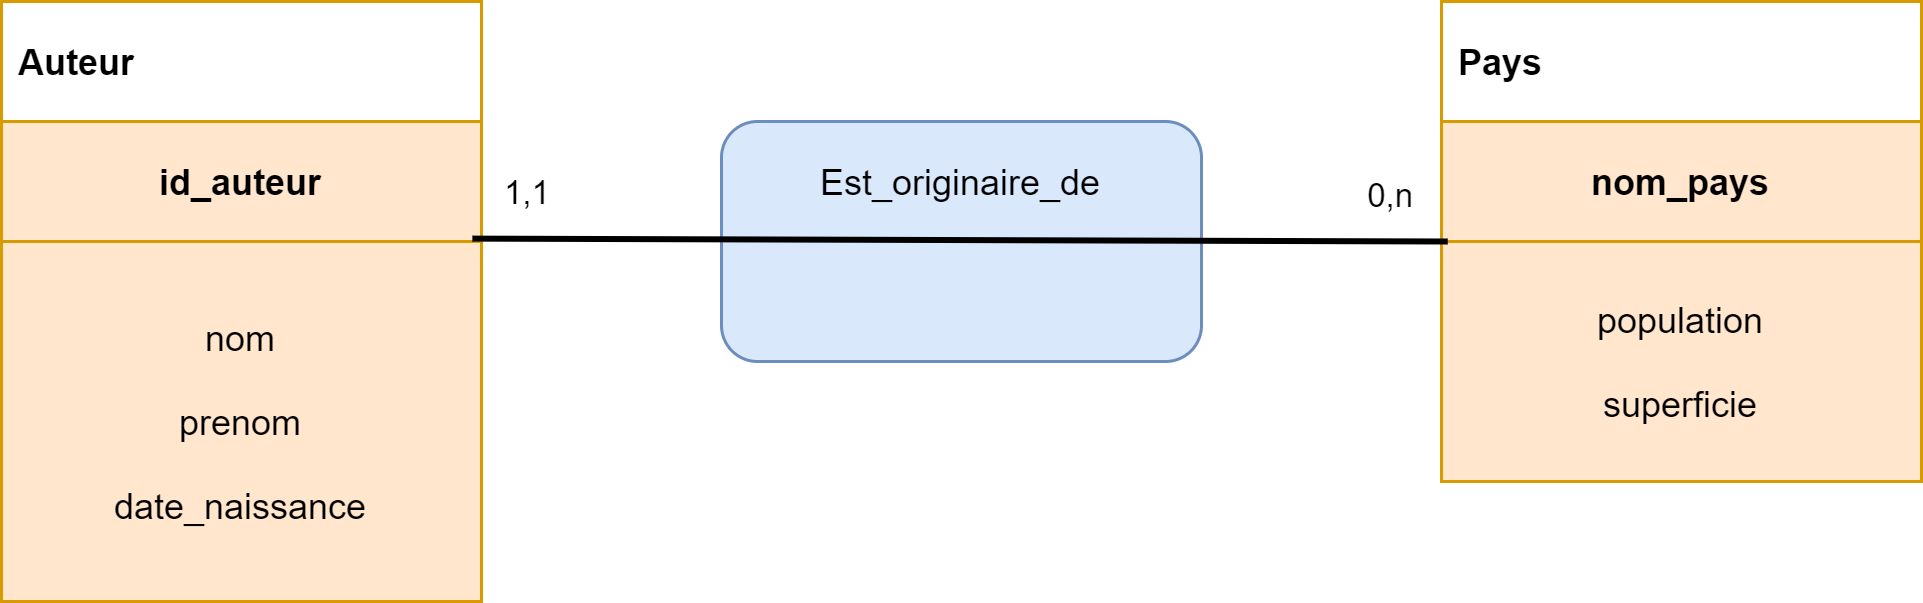
\includegraphics[width=11cm]{img/schema_1}
    \end{center}
    Une cardinalité est un couple d'entiers « de type $\min, \max$» :
    \begin{itemize}
        \item	la cardinalité 1,1 signifie qu'un auteur peut être lié au minimum à 1 pays, et au maximum à 1 pays (donc à un pays et un seul) ;
        \item	la cardinalité 0,n signifie qu'un pays peut être lié au minimum à aucun auteur et au maximum plusieurs auteurs.
    \end{itemize}
\end{exemple}


\subsection{Un schéma abouti}
\begin{center}
    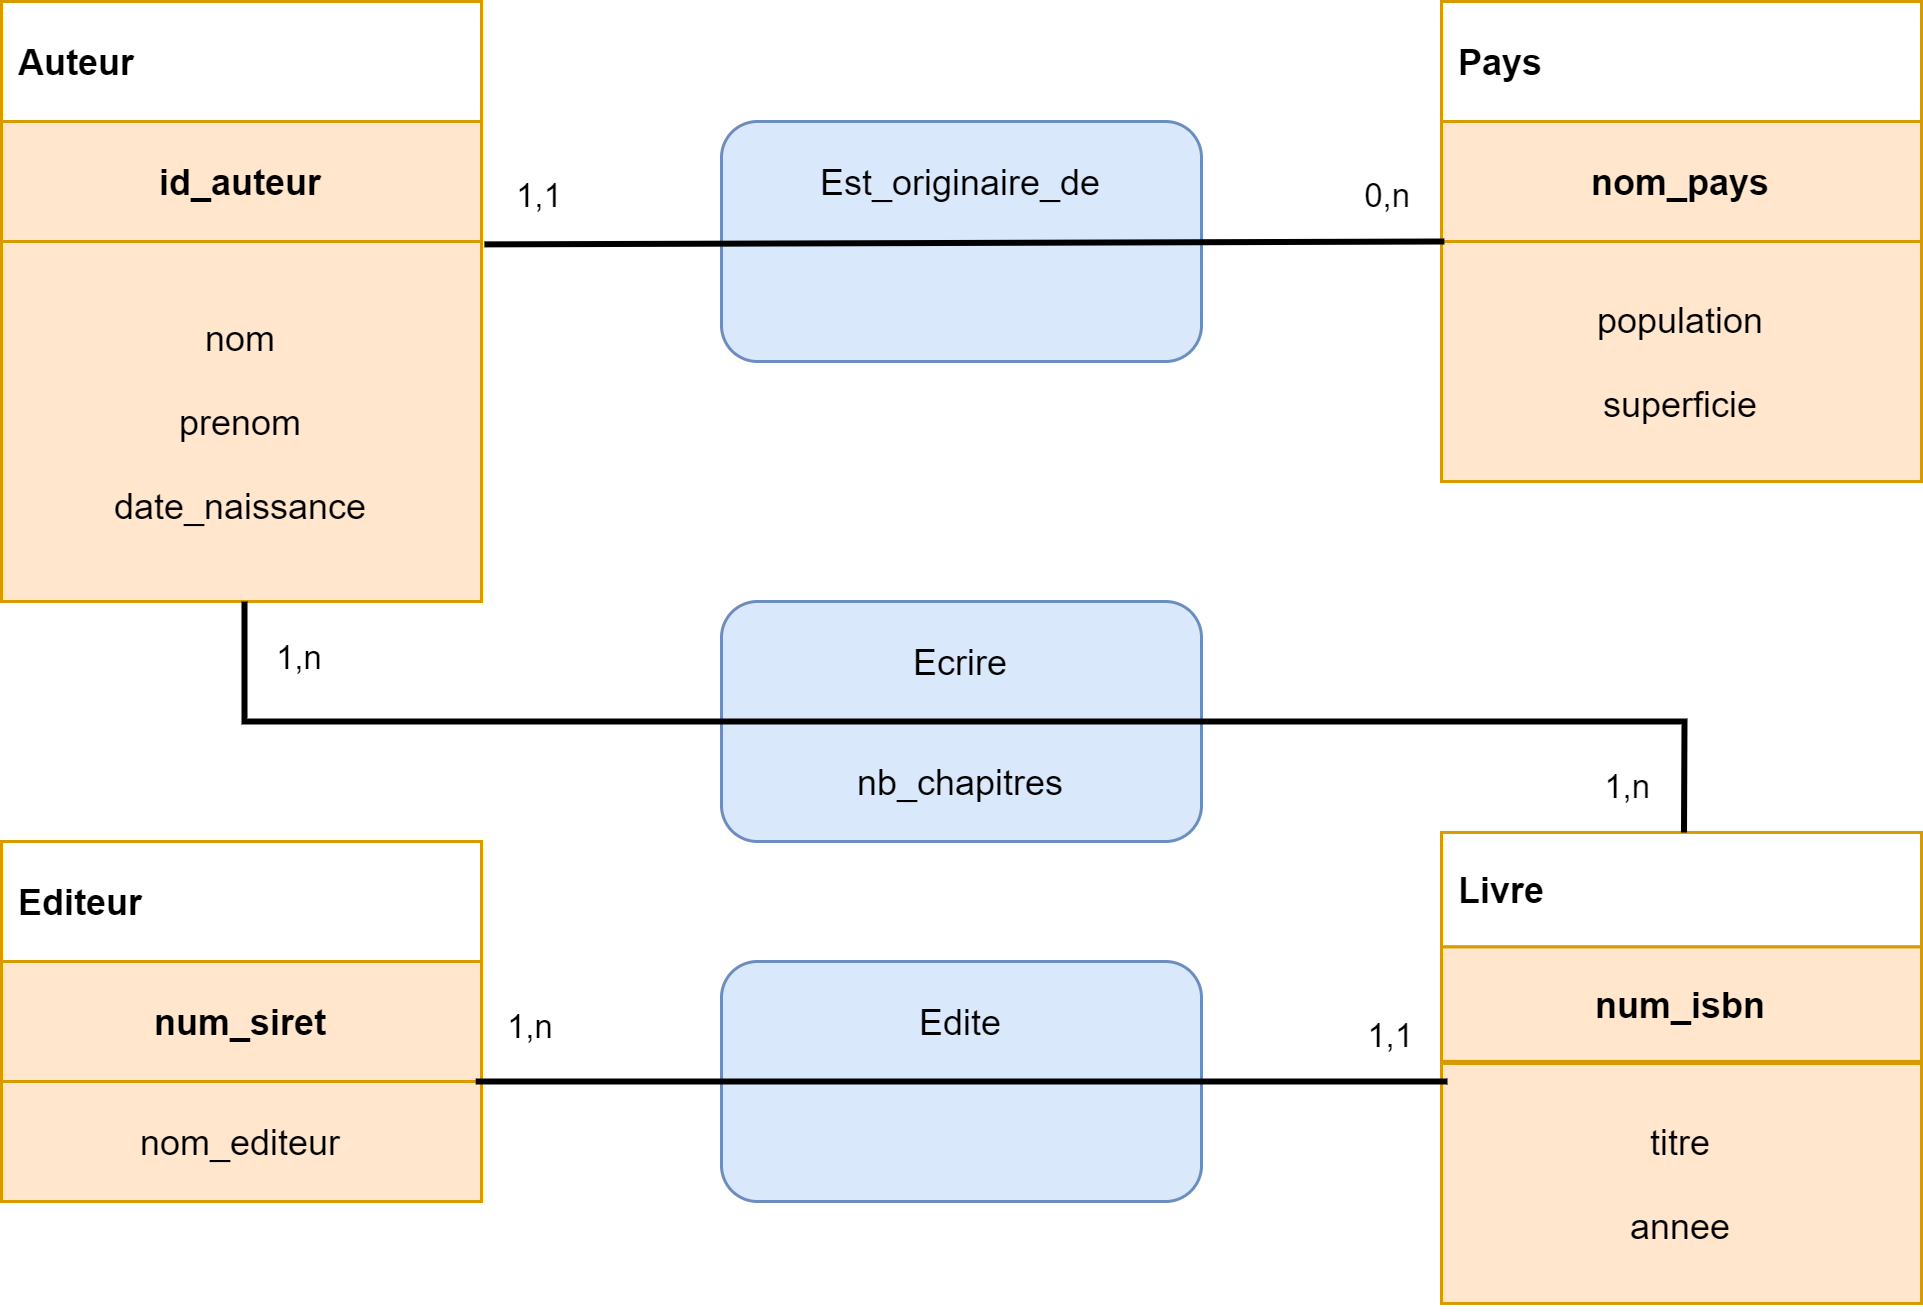
\includegraphics[width=11cm]{img/schema_2}
\end{center}

\subsection{Non-unicité des schémas}
Le schéma précédent s'appelle un modèle conceptuel des données (MCD).\\
On peut modéliser une situation avec plusieurs MCD, chacun d'entre eux ont leurs avantages et leurs inconvénients.

\section{Exercices}

\begin{exercice}[]
    \begin{center}
        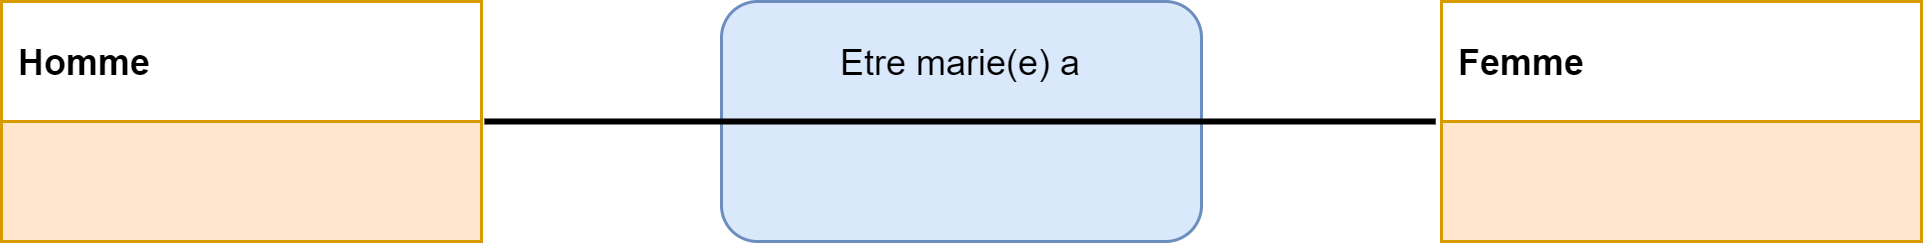
\includegraphics[width=12cm]{img/ex1}
    \end{center}
    Préciser les cardinalités de l'association \textit{Etre marie(e) a} :
    \begin{itemize}
        \item 	dans une société monogame ;
        \item 	dans une société dans laquelle les femmes ont le droit d'être polygames.
    \end{itemize}
\end{exercice}

\begin{exercice}[]
    \begin{center}
        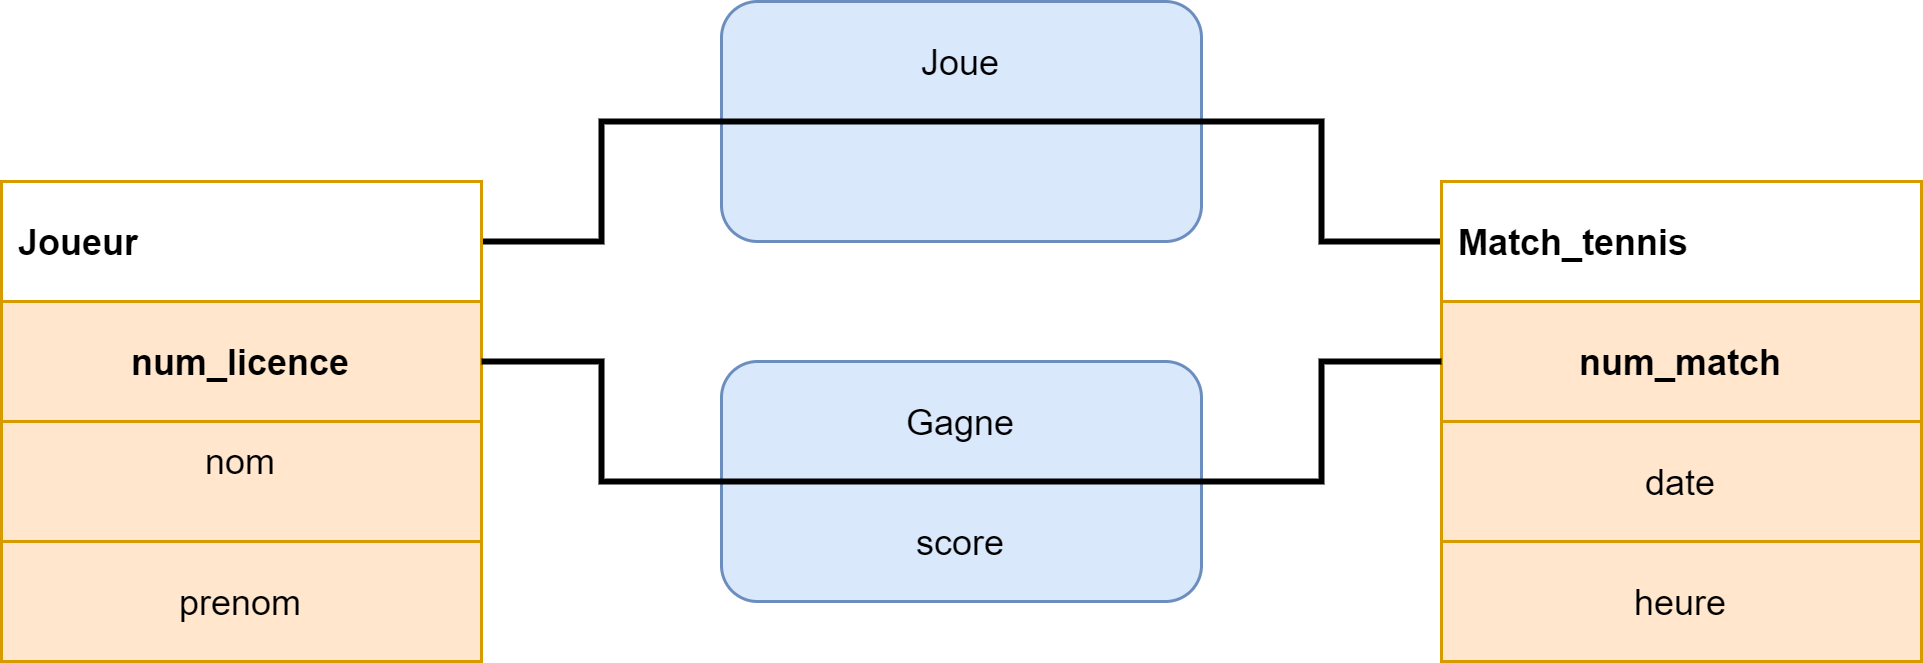
\includegraphics[width=12cm]{img/ex2}
    \end{center}
    Préciser les cardinalités des associations.
\end{exercice}
\newpage

\begin{exercice}[]
    \begin{center}
        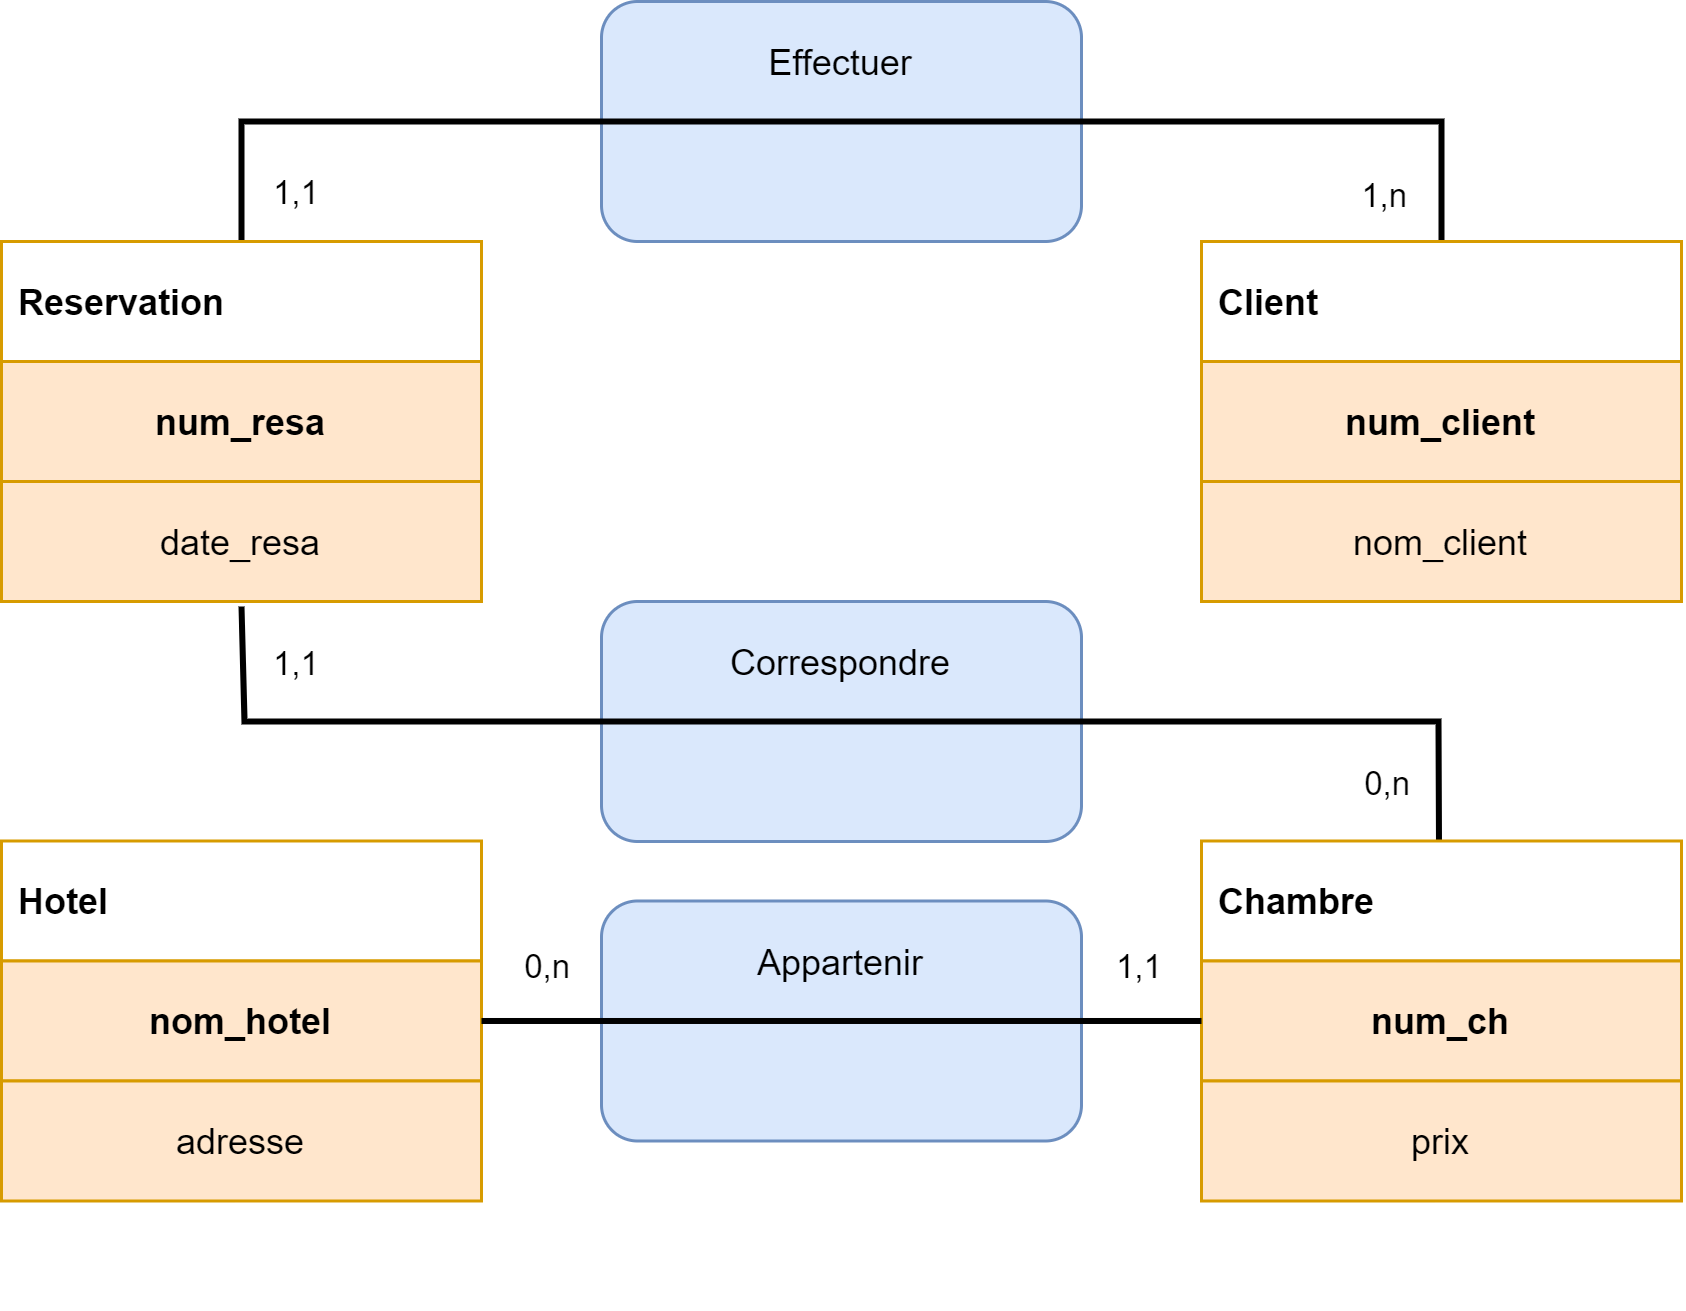
\includegraphics[width=12cm]{img/ex_hotel}
    \end{center}
    Dans ce modèle
    \begin{enumerate}
        \item 	Peut-on avoir des clients homonymes ?
        \item 	Un client peut-il réserver plusieurs chambres à une même date ?
        \item 	Est-il possible de réserver une chambre plusieurs jours d'affilée ?
        \item 	Peut-on savoir si une chambre est libre à une date donnée ?
        \item 	Peut-on réserver la même chambre plusieurs fois à la même date ?
    \end{enumerate}
\end{exercice}
\newpage
\begin{exercice}[]
    \begin{center}
        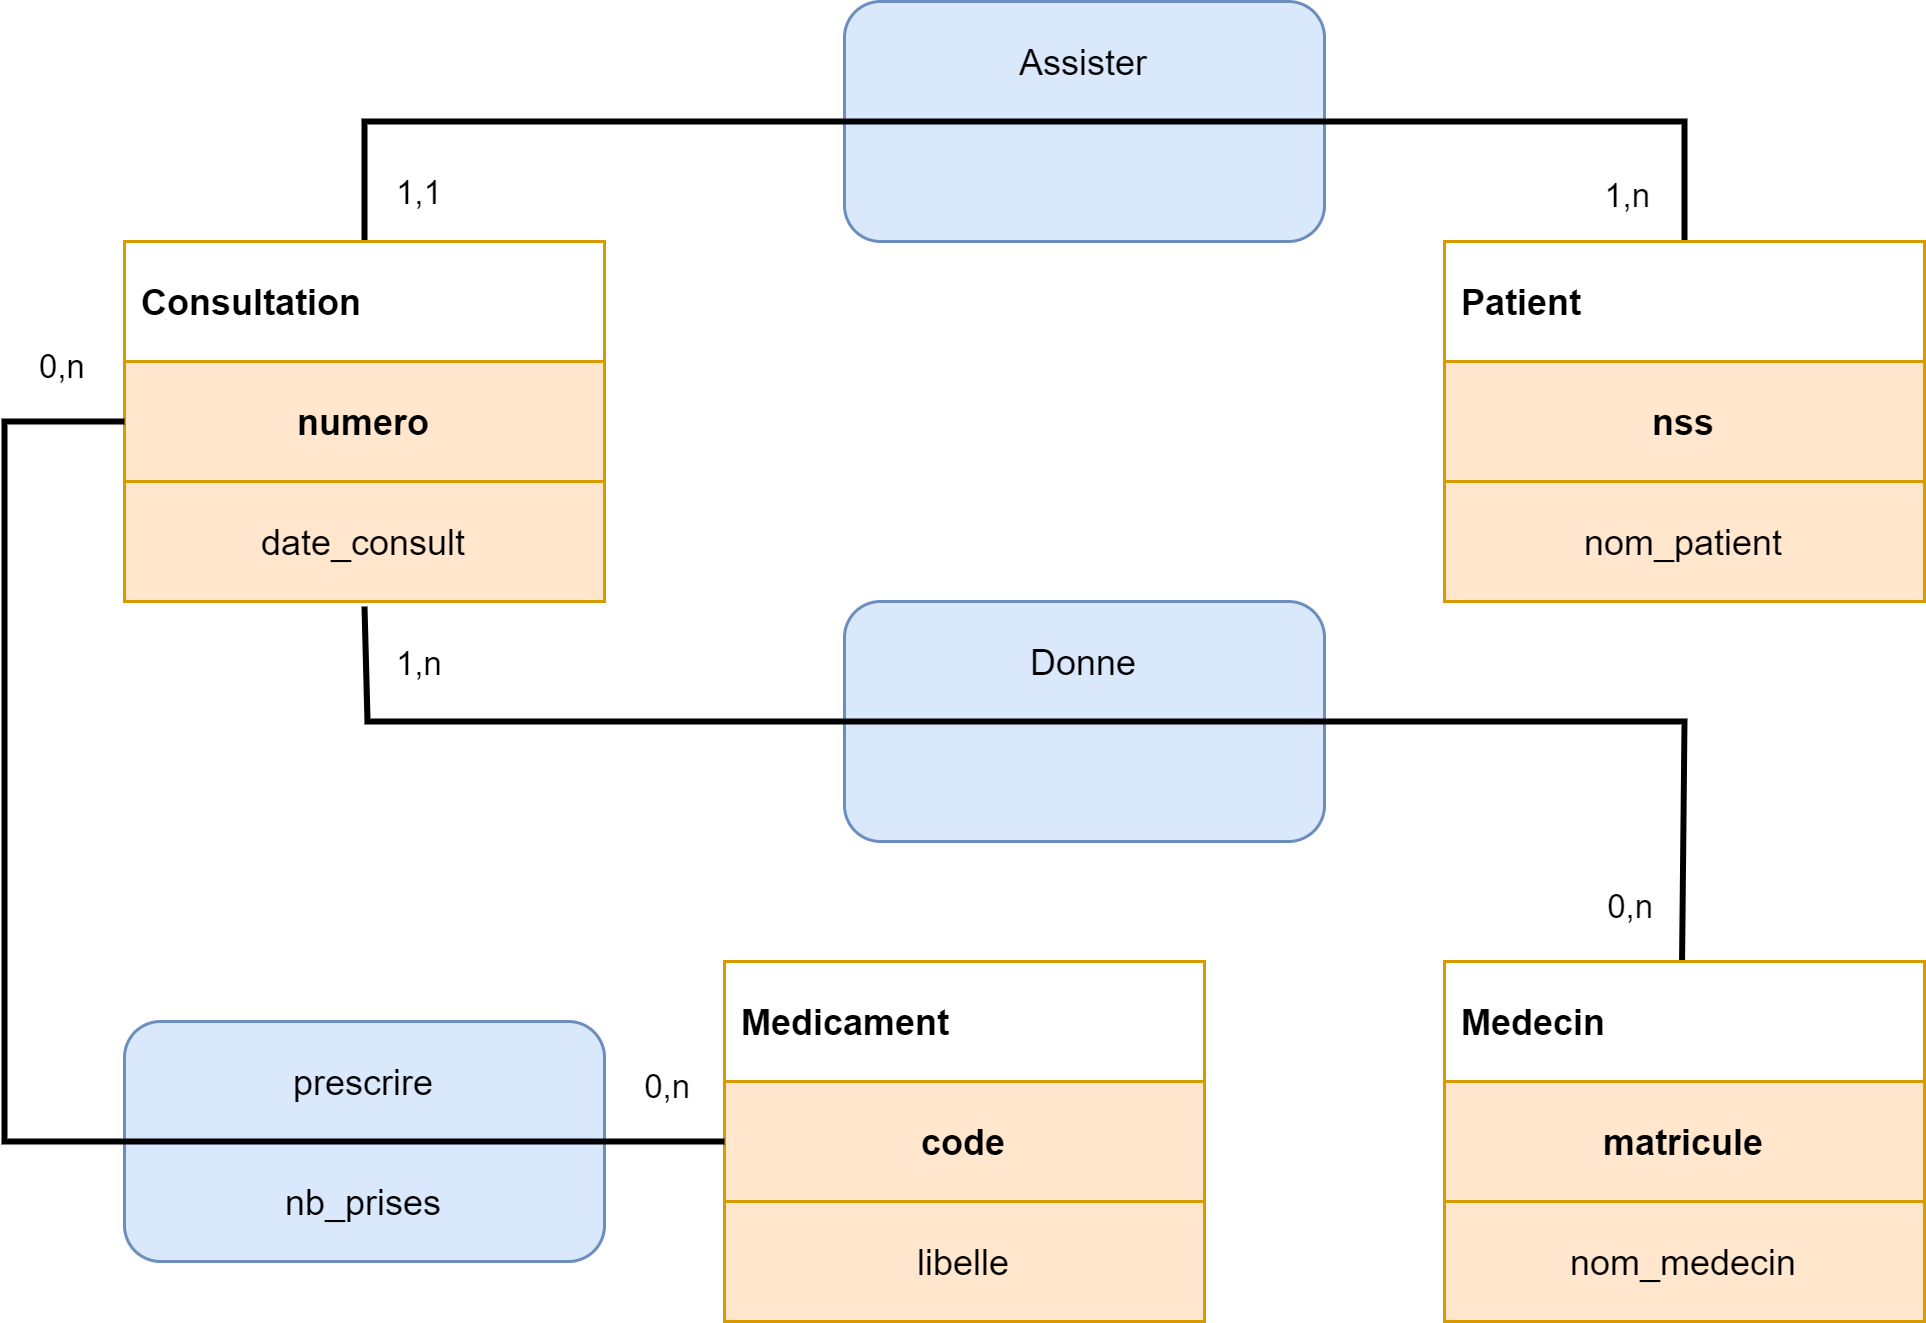
\includegraphics[width=12cm]{img/ex_consultation}
    \end{center}
    Dans ce modèle
    \begin{enumerate}
        \item 	Un patient peut-il assister à plusieurs consultations ?
        \item   Deux patients peuvent-ils assister à la même consultation ?
        \item   Deux consultations peuvent-elles avoir lieu le même jour ?
        \item 	Un médecin peut-il recevoir plusieurs patients lors d'une même consultation ?
        \item   Plusieurs médecins peuvent-ils assister à la même consultation ?
        \item   Une consultation entraîne-t-elle toujours une prescription ?
        \item 	Peut-on prescrire plusieurs médicaments lors d'une même consultation ?
        \item   Deux médecins différents peuvent-ils prescrire le même médicament ?
        \item   \'Etant donné un médicament prescrit, peut-on toujours connaître le médecin qui l'a prescrit ?
              
    \end{enumerate}
\end{exercice}


\begin{exercice}[]
    Une entreprise est identifiée par son nom.\\
    Dans cette entreprise, un département est identifié par un nom et caractérisé par une localisation.\\
    Un employé est caractérisé par un numéro, son nom, son grade et le département dans lequel il travaille.\\
    Le numéro d'un employé est unique dans un département mais pas dans l'entreprise.\\
    Donner le MCD, en précisant les attributs.\\
    
    \textit{Indication : « caractérisé» fait référence à un attribut, « identifié» à un identifiant.}
\end{exercice}

\begin{exercice}[]
    \begin{center}
        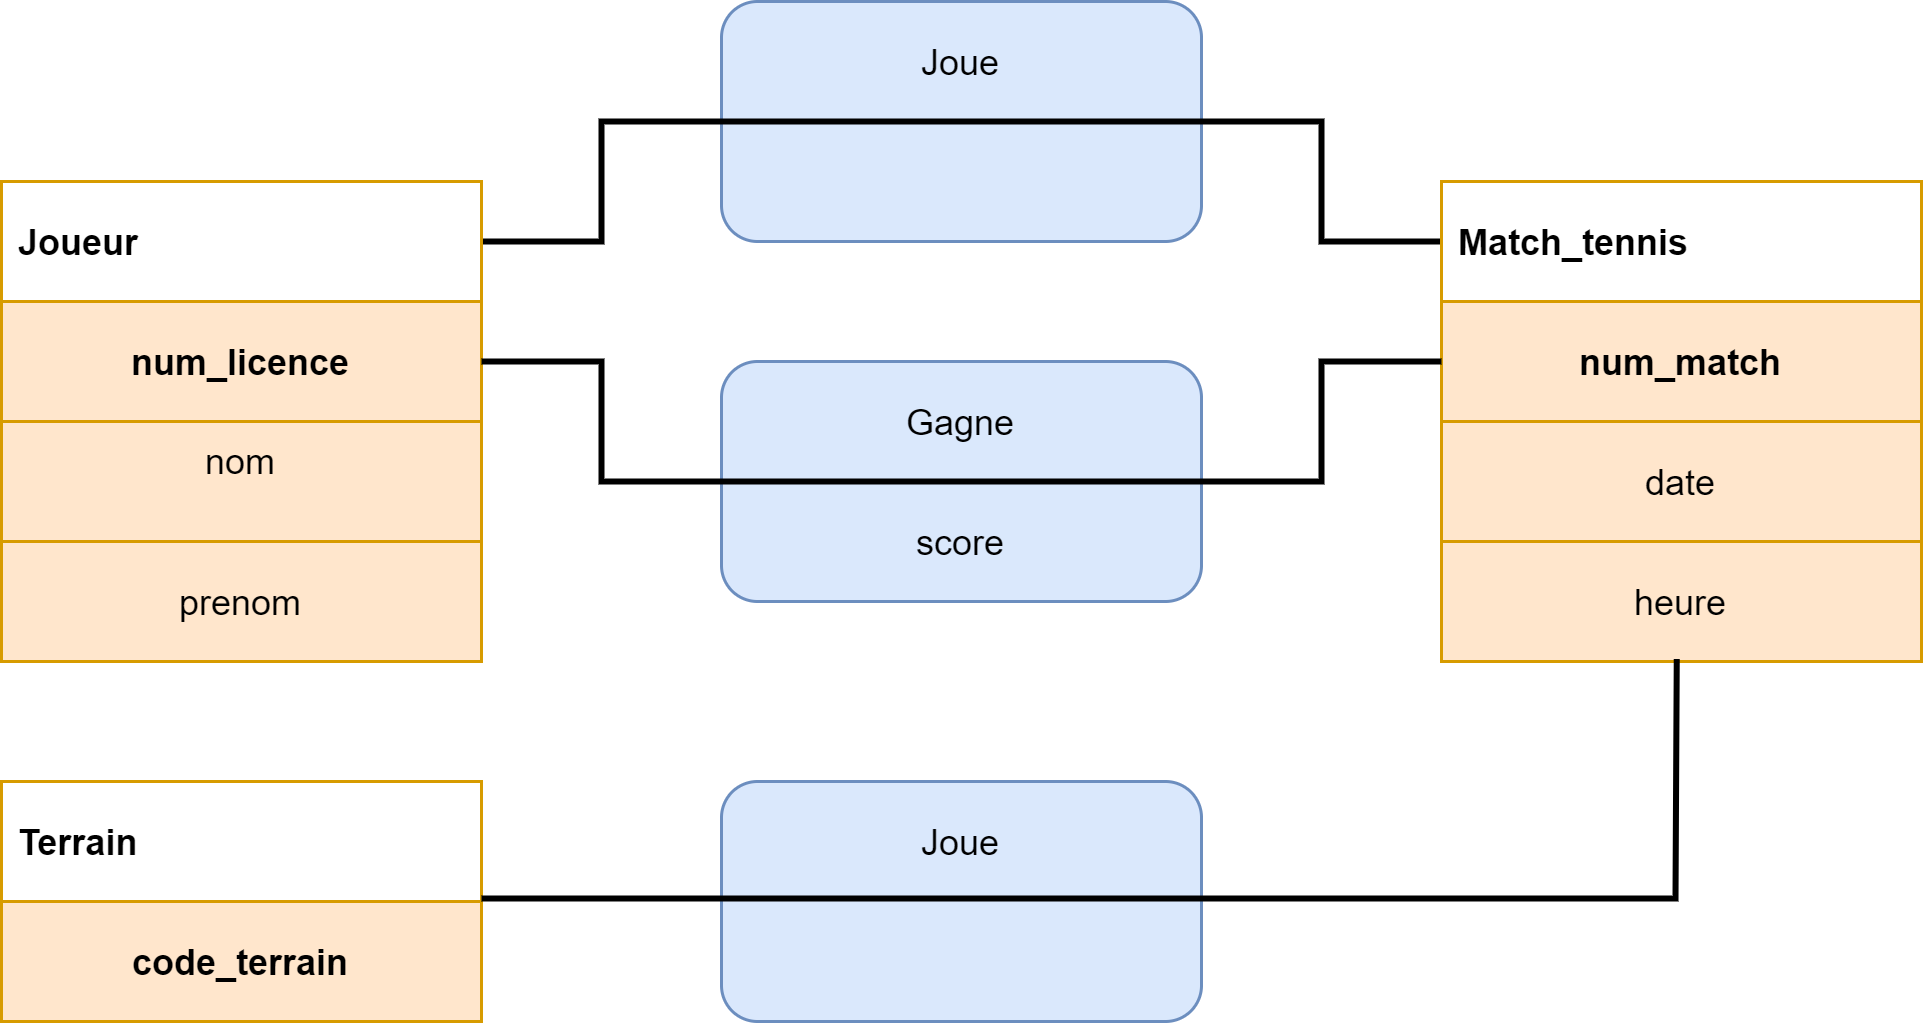
\includegraphics[width=12cm]{img/ex3}
    \end{center}
    \begin{enumerate}
        \item 	Reprendre les cardinalités du précédent MCD sur le tennis et préciser celle de \textit{Joue}.
        \item 	Selon ce modèle peut-on jouer des matchs de double ?
        \item 	Un joueur peut-il gagner un match sans y avoir participé ?
        \item 	Peut-il y avoir 2 matchs sur le même terrain à la même heure ?
        \item 	Connaissant un joueur, peut-on savoir sur quel(s) terrain(s) il a joué ?
    \end{enumerate}
\end{exercice}

\begin{exercice}[]
    On considère une médiathèque contenant des ouvrages pouvant être empruntés.\\
    Un ouvrage est caractérisé par un numéro unique, un titre, un auteur et un éditeur. En outre, on décrit un ouvrage par un certain nombre de mots-clés qui indiquent les sujets qui y sont traités.\\
    La médiathèque dispose d'un ou plusieurs exemplaires de chaque ouvrage, L'exemplaire est identifié par un numéro et caractérisé par sa position dans les rayonnages et sa date d'achat.
    Un exemplaire peut être emprunté par un emprunteur. Ces derniers sont identifiés par un numéro d'emprunteur et possèdent un nom et une adresse.\\
    
    Donner le MCD.
\end{exercice}
